% load packages!
\documentclass[12pt]{article}
\usepackage{caption}
\usepackage{setspace}
\usepackage{graphicx}
\usepackage{indentfirst}
\usepackage[margin=1in]{geometry}   
\usepackage{placeins}
\usepackage[square,sort,comma,numbers]{natbib}
\usepackage{float}
\usepackage[utf8]{inputenc}
\usepackage[T1]{fontenc}
\usepackage{csquotes}
\usepackage[stable]{footmisc}
\usepackage{hyperref}

% let's get this goin
\begin{document}

% make section headers less obnoxiously large, add italics
\makeatletter
\renewcommand\section{\@startsection {section}{1}{\z@}%
                                     {-1.5ex\@plus -1ex \@minus -.2ex}%
                                     {.75ex \@plus .2ex}%
                                     {\normalfont\normalsize\bfseries}}% 
\renewcommand\subsection{\@startsection{subsection}{2}{\z@}%
                                     {-1.0ex\@plus -1ex \@minus -.2ex}%
                                     {.5ex \@plus .2ex}%
                                     {\normalfont\normalsize\itshape}}%
\renewcommand\subsubsection{\@startsection{subsubsection}{3}{\z@}%
                                     {0 ex\@plus -.5ex \@minus -.1ex}%
                                     {0 ex \@plus .1ex}%
                                     {\normalfont\normalsize\itshape}}%
\makeatother

% add the title, author, date
\title{\vspace{-10pt} Gender, Code Documentation, and Communities of Statistical Computing}
       
\author{\textit{Simon Couch—16 December 2019}}

\date{}

\maketitle

% set spacing a bit larger
\doublespace

% input each section TeX file
\section{Introduction}\label{sec:intro}

Occupational sex segregation remains resilient in the United States despite the significant economic benefits shown to be associated with integration \cite{sex_seg}. Rather than attributing these gaps in representation completely to discrimination or coercion on the part of employers, recent scholarship also articulates supply-side mechanisms for occupational sex segregation, showing how ``the reproduction of occupational sex segregation [is in part due to] the deeply personal, self-reflective---yet culturally and structurally gendered---career decision making of men and women'' \cite{cech_self-expressive_2013}. Rather than regarding ``interest'' in careers as inherent to individuals, this literature demonstrates how self-expression is part and parcel of gendered socialization. In this paper, I will show how these mechanisms come to bear on individuals pursuing careers in statistical computing. Specifically, I examine two user communities formed around the R programming language, and how the representation of gender minorities in these communities is deeply interconnected with practices of code documentation prevalent among them. Rather than conceptualizing code documentation as unargumentative or ideologically neutral, I argue that these resources are capable of delivering feedback to readers about their competence and identity alignment with careers in computational statistics and, further, that this is especially consequential for readers whose identities do not align with their conceptualization of the typical worker.

\section{Literature Review}\label{sec:scholarly}

\subsection{Supply-Side Arguments of Gendered Occupational Segregation}

Over the past two decades, the body of sociological and social-psychological literature characterizing supply-side mechanisms for gendered occupational segregation has progressed significantly. In contrast to demand-side arguments, which examine the effect of discrimination and bias at the institutional and interactional level, supply-side arguments characterize the forces which ultimately lead to the ``subconscious gendering of men’s and women’s self-expressive career decisions'' \cite{cech_self-expressive_2013}. The focus, then, is not on how applicants are recruited and evaluated, but rather on the processes funneling individuals into gender-typed degree programs, social organizations, and applicant pools, and the mechanisms by which these processes are disguised as ``self-expression.'' (It is worth noting that arguments for supply-side and demand-side dynamics are not necessarily in opposition, but instead come together to collectively contribute to more diversified inequality regimes.) A key process noted in the literature on supply-side dynamics is the role of status generalizations for self-perceptions of competence and belonging; these works argue that gendered cultural beliefs inform the extent and manner in which individuals incorporate feedback into evaluations of their own ability and fit in gendered occupational fields. Specifically, I trace the literature relevant to supply-side mechanisms affecting gender minorities in technical fields in the last two decades, which collectively shows that gender minorities are subject to greater marginalization and negative feedback in their educational paths to technical fields than straight cis-men, and further, that they are more likely to incorporate this negative feedback into their self-perceptions, resulting in greater attrition from these educational sequences (and by extension inadequate representation in the applicant pool.)  
	
Correll argued in 2001 that, controlling for actual ability, individuals’ self assessments of their competence in gendered career-relevant tasks are influenced by cultural beliefs about gender. Specifically, this longitudinal observational study showed that eighth-grade through college-aged women perceived themselves as less competent at math (argued to be a highly masculine-typed skillset) and more readily incorporated feedback (in the form of standardized test-taking performance) into their self-perceptions of their mathematical ability than men. These effects did not manifest identically for verbal skills, instead showing that men rated themselves as similarly competent on average, yet were more prone to incorporate negative feedback into their self-perceptions of their own ability in this area, showing that this phenomenon is generalizable beyond women in masculine-typed fields. More generally, then, ``the appraisals individuals make of their own competence at various tasks are more contingent on local evidence when societal expectations for success are lacking.'' Further, in this study, Correll finds that more positive self-assessments result in greater chances of persisting on a given career path, even after controlling for ability (as measured through test-taking performance.) These findings, taken together, articulate a supply-side mechanism for unequal representation in the candidate field for gendered occupations \cite{correll_gender_2001}.   

In 2004, Correll furthered her argument on this mechanism by implementing it in an experimental setting. After exposing undergraduate subjects to beliefs that men were more competent at a given task, she found that the men subjects assessed their own ability more highly than women and were more likely to express interest in careers for which men were supposedly more fit for. These effects disappeared when subjects were instead exposed to egalitarian views. Through the use of experimental methodology, Correll further supports her earlier argument that people’s self-perceptions of their abilities in gender-typed skillsets are influenced by cultural gender beliefs and, further, that individuals more readily incorporate feedback into their self-perceptions when they confirm beliefs perceived to be widely held about gendered task competence. These studies were foundational for developing understandings of the way that ``status generalization occurs in individual evaluative settings'' in that self-evaluation is indeed social to the extent that people utilize status characteristics to inform their relative position in some greater collective \cite{correll_constraints_2004}.  

Hargittai and Shafer implement a similar experimental approach in a 2006 paper on web-use skills. In this study, the authors do not find differences between men and women in ability to navigate online content. However, women participants rated their own Web-use skills, defined as the ability to locate information and resources on the internet, significantly lower than men. The authors hypothesize that this difference in self-perception could lead to significant disparities in both absolute exposure to internet use as well as the kind of content that participants engage with. This research shows that the online setting itself is a gendered context in regard to self-evaluation, even without the presence of task assignments which are themselves gendered outside of an internet context \cite{hargittai_differences_2006}. While the task of basic information-finding on the internet might seem dated, these findings are particularly relevant to the practice of navigating technical documentation. Especially within the base-R environment, many resources and help-files, as well as the pathways to locate them, have not changed since the publishing of this study in 2006. Even in the context of a tidy based workflow, interaction with the R console and RStudio IDE in searching for relevant and informative documentation presents a task that is arguably more reminiscent of early internet resource-finding than modern Web-surfing.  

In 2011, Cech et al. furthered these understandings of how individual evaluations are informed by status generalization to beget a supply-side mechanism for gendered occupational segregation. The study found that, once engineering undergraduates selected their major, their self-perceptions of their own competence in engineering did not significantly influence their intent to remain in the field. The study also disconfirms previous hypotheses that women are more likely to consider family plans when choosing careers, thus resulting in aspirations for more female-typed occupations that are more likely to have normative cultures or significant policy centered on accomodating families. Instead, as the mechanism explaining how individuals choose—and decide whether to remain in—gendered occupations, the authors propose a mechanism that they name professional role confidence, focusing not only on individuals’ self-perceptions of actual competence, but also in their ability to fulfill roles and identity features associated with gendered occupations. Professional role confidence was shown to be especially pivotal for persistence in pursuit of gendered-occupations. Further, the authors argued that women have less professional role confidence in general and that this disparity is amplified in engineering and other masculine-typed occupations \cite{cech_professional_2011}.  

Another instance of this professional role confidence at play was articulated two years earlier by Cheryan et al. Again moving beyond self-evaluation of skillsets as a mechanism for generating career interest, Cheryan et al. argued a theory of \textit{ambient belonging} in 2009, in that individuals use cues from their physical environment to inform their professional role confidence. Focusing on women interested in computer science, the authors conduct a series of studies demonstrating that ``stereotypes can be communicated (and altered) merely through the physical cues present in an associated environment,'' and further that the demasculinization of the physical environment is ``sufficient to boost female undergraduates’ interest in computer science to the level of their male peers'' \cite{cheryan_2009}. This series of studies articulates another supply-side mechanism for gendered occupational choice, where gender minorities not only differentially incorporate feedback and evaluation into their self-perceptions of their belonging in a gendered occupation, but also gendered environmental cues.

In a series of recent papers, Cech and coauthors have extended gendered understandings of supply-side mechanisms beyond the cis-binary in studies of the experiences of gender minorities in undergraduate engineering programs and STEM-related government agencies. (My use of the term gender minorities here might be, in some ways, more evocative of gendered minorities; I include, in addition to people whose gender identity is inadequately represented in a given context, people who identify as lesbian, gay, bisexual, or any other non-heterosexual sexual orientation in acknowledgement that the lived experiences of people holding these identities differ from those of people identifying as straight in regard to the way that they are socialized as gendered individuals.) Initially, in an analysis of data from several federal agencies, the authors found that LGBT employees in governmental STEM organizations reported significantly lower job satisfaction and had higher turnover rates than their straight, cisgender colleagues \cite{cech_queer_2017}. More recently, Cech and Rothwell replicated this study with a larger sample across a greater number of federal agencies, this time exclusively those which have LBGT-inclusive policies. Results were consistent with previous research, though they incorporated an intersectional approach into their methods with racial and racial-interactive effects \cite{cech_lgbt_2019}. From a supply-side standpoint, these studies show that gender minorities are less likely to remain in STEM fields even after their entry into the workforce, exaggerating the already significant occupational segregation due to differences in career longevity. In 2018, Cech and Rothwell examined cultures of inclusivity—and their effects on individual self-perception—at eight U.S. engineering schools. The study found a persistent negative climate for gender minorities across each of the schools, arguing that this was indicative of educational institutions’ mirroring of predominant workplace cultures. This negative climate manifested both in the devaluation of work produced by gender minorities and in measures of social marginalization \cite{cech_lgbtq_2018}. This finding is especially consequential in light of Correll’s earlier works arguing that people differentially incorporate this negative feedback into their self-perceptions of their competence in accordance with dominant cultural gender beliefs. Doubly, under Cech’s framework of professional role confidence, even if gender minorities do not see this discriminatory treatment as reflective of their actual capabilities, their exposure to this climate could significantly affect their representation in the applicant pool through their perceptions of their ability to fulfill the roles and identity features associated with a given role-incumbent schema \cite{gorman_gender_2005}.  

Recent literature has demonstrated the continuing disadvantageous treatment that gender minorities face in undergraduate STEM education. For instance, in their 2017 paper, Blair et al. argue that the sampled STEM faculty predominantly characterize their gender conceptualizations as gender blind or gender acknowledging, both of which hold that ``interventionist positions to promote gender equity [are] inappropriate'' and places ``action to support gender equity outside the scope of their duties as faculty members.'' In refusing to engage in proactively disrupting bias in their curricular design, these faculty continue to engage in pedagogical practices catering to socialized hegemonic masculinity \cite{ohland_race_2011}. In 2015, Seron et al. argue that practices of professional socialization which are predominant in undergraduate engineering programs act as another mechanism for the reproduction of sex segregation. Specifically, the emphasis on collaborative work, though more reflective of professional engineering contexts, is argued to interact harmfully with gendered individual self-perceptions, as well as the differential incorporation of feedback confirming gendered cultural stereotypes, wherein women are made to explicitly negotiate ``assessing where one fits into the pecking order'' in men-dominated groups. Further, emphasized exposure to internship and shadowing experiences narrow gender minorities’ understanding of role-incumbent schemas in professional contexts, challenging their professional role confidence and, as I argued earlier, consequently decreasing their representation in these fields \cite{seron_persistence_2016}. Again, in light of Correll and Cech’s arguments described above, the findings of these studies are especially crucial for understanding retention of gender minorities in technical fields. Given that these populations differentially incorporate performance feedback and socialization into their self-perceptions of their own competence and belonging, and the demonstrated salience of these evaluations for career-path persistence, the (unsatisfied) need for inclusive STEM classroom cultures is made clear.  

The literature on supply-side mechanisms for gendered occupational segregation in the last two decades collectively articulates a powerful mechanism for the exclusion of gender minorities from STEM fields. Taken together, the outlined body of work shows that gender minorities continue to be subject to greater disadvantageous treatment throughout their educational paths to technical fields. Further, it is shown that this negative feedback is more likely to be incorporated into gender minorities’ self-evaluations of their ability and belonging, and that these accumulated socialized differences in self-perception measurably impact resilience in educational attainment.   

It is through this lens that I approach documentation practices in statistical computing. At the intersections of statistics and computer science, statistical computing is deeply embedded in—and draws methodological and cultural elements from—each of science, technology, engineering, and math. In this way, the social theory developing supply-side mechanisms for occupational gender segregation, and its application to understanding gender minorities’ representation in STEM fields, is relevant for understanding the representation of gender minorities in statistical computing.  

\subsection{R, RStudio, \& the tidyverse}\label{sec:tidy}

% The language
\textit{R} is an open-source programming language designed for statistical computing, and it is widely used across contexts ranging from academic research to business analytics to introductory statistics classes. At the time of writing, the first versions of the language were released over 25 years ago, and the language has been under active development since then. 

% CRAN
The stock capabilities of R are supplemented by a large body of user-created \textit{packages}, which are collections of code libraries (often containing \textit{functions}, which are code snippets that allow users to automate common tasks), datasets, and combinations of both. 

The founding of the \textit{Comprehensive R Archive Network (CRAN)} coincided with the first public beta release of the language in 1997. CRAN serves to facilitate this community development,  hosting packages in a common repository for all R users to freely download and modify. At the time of its initial release, CRAN hosted 12 packages; it now hosts over 15,000 \cite{cran}.

% RStudio
In 2011, an integrated development environment (IDE) called \textit{RStudio} was released for the language, providing users with a graphical interface to more easily interact with the language. The software is free for individual users, but commercial and server licenses are paid. A substantial proportion of R development occurs within RStudio, and one of the major R user conferences, \textit{rstudio::conf}, is hosted by the company.

% tidyverse
In 2014, Hadley Wickham, a prominent data scientist, formalized what he called \textit{tidy} data---tabular datasets ``where each column is a variable, each row is an observation, and each cell contains a single value'' \cite{wickham2014tidy}. Wickham developed and continues to develop a collection of packages built around this shared principle of data representation, providing tools to transform data into a tidy format, and further to extract meaning from data after it is ``tidied.'' The development of this collection of packages, which came to be known as the \textit{tidyverse}, now includes contributions from hundreds---if not thousands---of individual contributors of open-source code. Throughout this paper, I refer to tidy packages and non-tidy packages. In reality, this boundary is not obvious; while there is a concrete (yet adapting) set of packages formally included in the tidyverse, a substantial portion of tidyverse-unaffiliated package development still aligns to tidy data principles. I address the implications of this boundary work more thoroughly in Section \ref{sec:disc}.

% RStudio and tidyverse alignment, capitalism
Notably, though, the tidyverse is largely a product of RStudio. Dr. Wickham has been employed by the company since January 2013 \cite{wickhamhadley}, and the company employs several prominent R data scientists full-time who, almost exclusively, contribute open-source code to improve package functionality in---and to promote---the tidyverse \cite{rstudiopackages, future_r_hadley}.

% tidyverse and Inclusivity
The R community, especially the tidyverse, has been regarded as a much more inclusive and diverse group of users than that which utilizes competing data science toolkits such as Python---a 2015 study estimated that 9.2\% of R package authors are women, whereas 2\% of Python package authors are women \cite{mair2015motivation}. In a recent interview, Dr. Reshama Shaikh, a prominent data scientist and organizer for women in the field, said that, compared to the Python community, the R community is ``really relaxed, and fun, and welcoming'' \cite{shaikhwomen2019}. Similarly, in a recent interview, Dr. Wickham noted that ``people tell me they love R because the community is so welcoming. I think a large part of that is because of that it has become much more diverse'' \cite{future_r_hadley}. Dr. Shaikh notes that she believes an essential element of fostering this culture took place through coordinated, collective organization:

\begin{displayquote}
``Everyone is committed to diversity. Everybody wants inclusivity, and they're all working hard, and they all have initiatives, but when I looked at the Python community, it's like each group is in its own individual kayak and they're rowing hard, everyone's looking at the same direction and they're moving there and they're all working hard, but the R community has sort of invested in this really large boat and they can move to their goal a lot faster with a lot less rowers to get where they want to go'' \cite{shaikhwomen2019}.
\end{displayquote}

This community coordination is driven by two primary organizing forces: the R-Ladies organization and RStudio (and by extension, then, the tidyverse.) Founded in 2012, R-Ladies ``is a global grassroots organisation whose aim is to promote gender diversity in the R community'' \cite{grieves}. R-Ladies has had a profound and widespread impact on representation of gender minorities in the R user community, and its membership is indicative of gender representation by programming language; while it is estimated that there are more than six times as many users of Python than users of R, the R-ladies organization has almost 30,000 members, while PyLadies (the analogous gender diversity advocacy group for Python) has only 36,500 members \cite{shaikhblog}. Wickham recently reflected on RStudio's unique position as a for-profit company to make an impact on the community to which it markets to in a recent interview.

\begin{displayquote}
``There is also this broader question about how we make sustainable open-source software. Companies get this huge economic benefit from it, and they are not required to give back. It’s very hard to rely on philanthropy, so how do we extract some of the economic value open-source is generating and reinvest it back into the community?'' \cite{future_r_hadley}.
\end{displayquote}

Much of the reinvestment that Wickham mentions takes place through the R Consortium, a collection of organizations ``chartered to fund and inspire ideas that will enable R to become an even better platform for science, research, and industry'' \cite{rstudio_about}. In 2018, the R Consortium announced that R-Ladies would be a named a top-level project, providing the organization with ``long term investment for success'' \cite{mertic_r}. In this way, the tidyverse community's investment in increasing representation of gender minorities becomes clear.

With this context in mind, I now examine the degree to which these conceptualizations of representation are reflected through code documentation.





\section{Methods}\label{sec:methods}

I use a mixed-method approach to understanding the inflection of gender through technical documentation. In Section \ref{sec:qual}, I describe the study's methodology in conducting interviews with notable figures from statistical computing in order to understand their conceptualizations of effective documentation, as well as the mechanisms responsible for differences in the way that documentation is structured and presented. Then, in Section \ref{sec:coa}, I describe my methods in conducting a class of object analysis, quantifying these differences in the presentation of code documentation arising from the two development communities described in Section \ref{sec:tidy}.\footnote{The implications of this boundary work delineating between tidyverse and non-tidyverse development are considered more critically in Section \ref{sec:disc}}.

\subsection{Qualitative Interviews}\label{sec:qual}

In order to validate a set of measures attempting to quantify documentation quality, and to more thoroughly investigate the relationship between representation of gender minorities and differences in documentation practices between the tidyverse and other R development communities, I conducted two interviews with women directly involved in this field. Specifically, both of my interviewees hold Ph.D.s in statistics, have taught computational statistics in some setting, and have made significant contributions to the tidyverse, tidyverse-adjacent R packages, or other statistical computing development projects. At the beginning of each interview, I asked for consent to record the interviewee's responses, as well as whether or not they wished to be identified in works resulting from the interviews; one interviewee requested that her responses remain anonymous. Due to the very small size of this sample space, I do not identify either interviewee by name, instead referring to them as interviewee $A$ and $B$. Each interview lasted roughly 30 minutes and was conducted using a semi-structured approach in order to ensure that certain topics were discussed while also allowing for elaboration and clarification on dicussion topics especially relevant to each interviewee. The interview protocol is included in Appendix \ref{sec:interview}.

\subsection{Class of Object Analysis}\label{sec:coa}

Making use of the criteria developed through conducting interviews, I analyze the documentation resources provided alongside software packages on CRAN. Specifically, I examine how the presentation of these resources differs between packages affiliated with the tidyverse (tidy packages) and those not affiliated (non-tidy packages.) R source code for all analyses presented is publicly available online.\footnote{Source code available at: \href{https://github.com/simonpcouch/gendering_documentation}{\textit{https://github.com/simonpcouch/gendering\_documentation}}}


\subsubsection{Data Acquisition} \hspace{10pt} In order to conduct this analysis, I first need to control for factors other than development community that might also contribute to differences in the structure of these resources. Most notably, as my interviewees noted, and as justified in Figure \ref{fig:users}, packages in the tidyverse have, on average, a substantially larger number of monthly downloads than those not in the tidyverse. In order to account for this difference, I use a matched-pairs sampling approach---since there are significantly fewer packages from the tidyverse than from the non-tidy community, I include every tidy package in my sample, and sample the package with the most similar number of package downloads in the last month to each tidy package.\footnote{I do not posit that the actual pairing of these packages is meaningful, but that the overall distribution of usership is important to approximate in order to control for package popularity and, by extension, resources available for maintenance and documentation improvement.}

\begin{figure} [!htb]
    \caption{Distribution of Usership by Development Community}
    \centering
    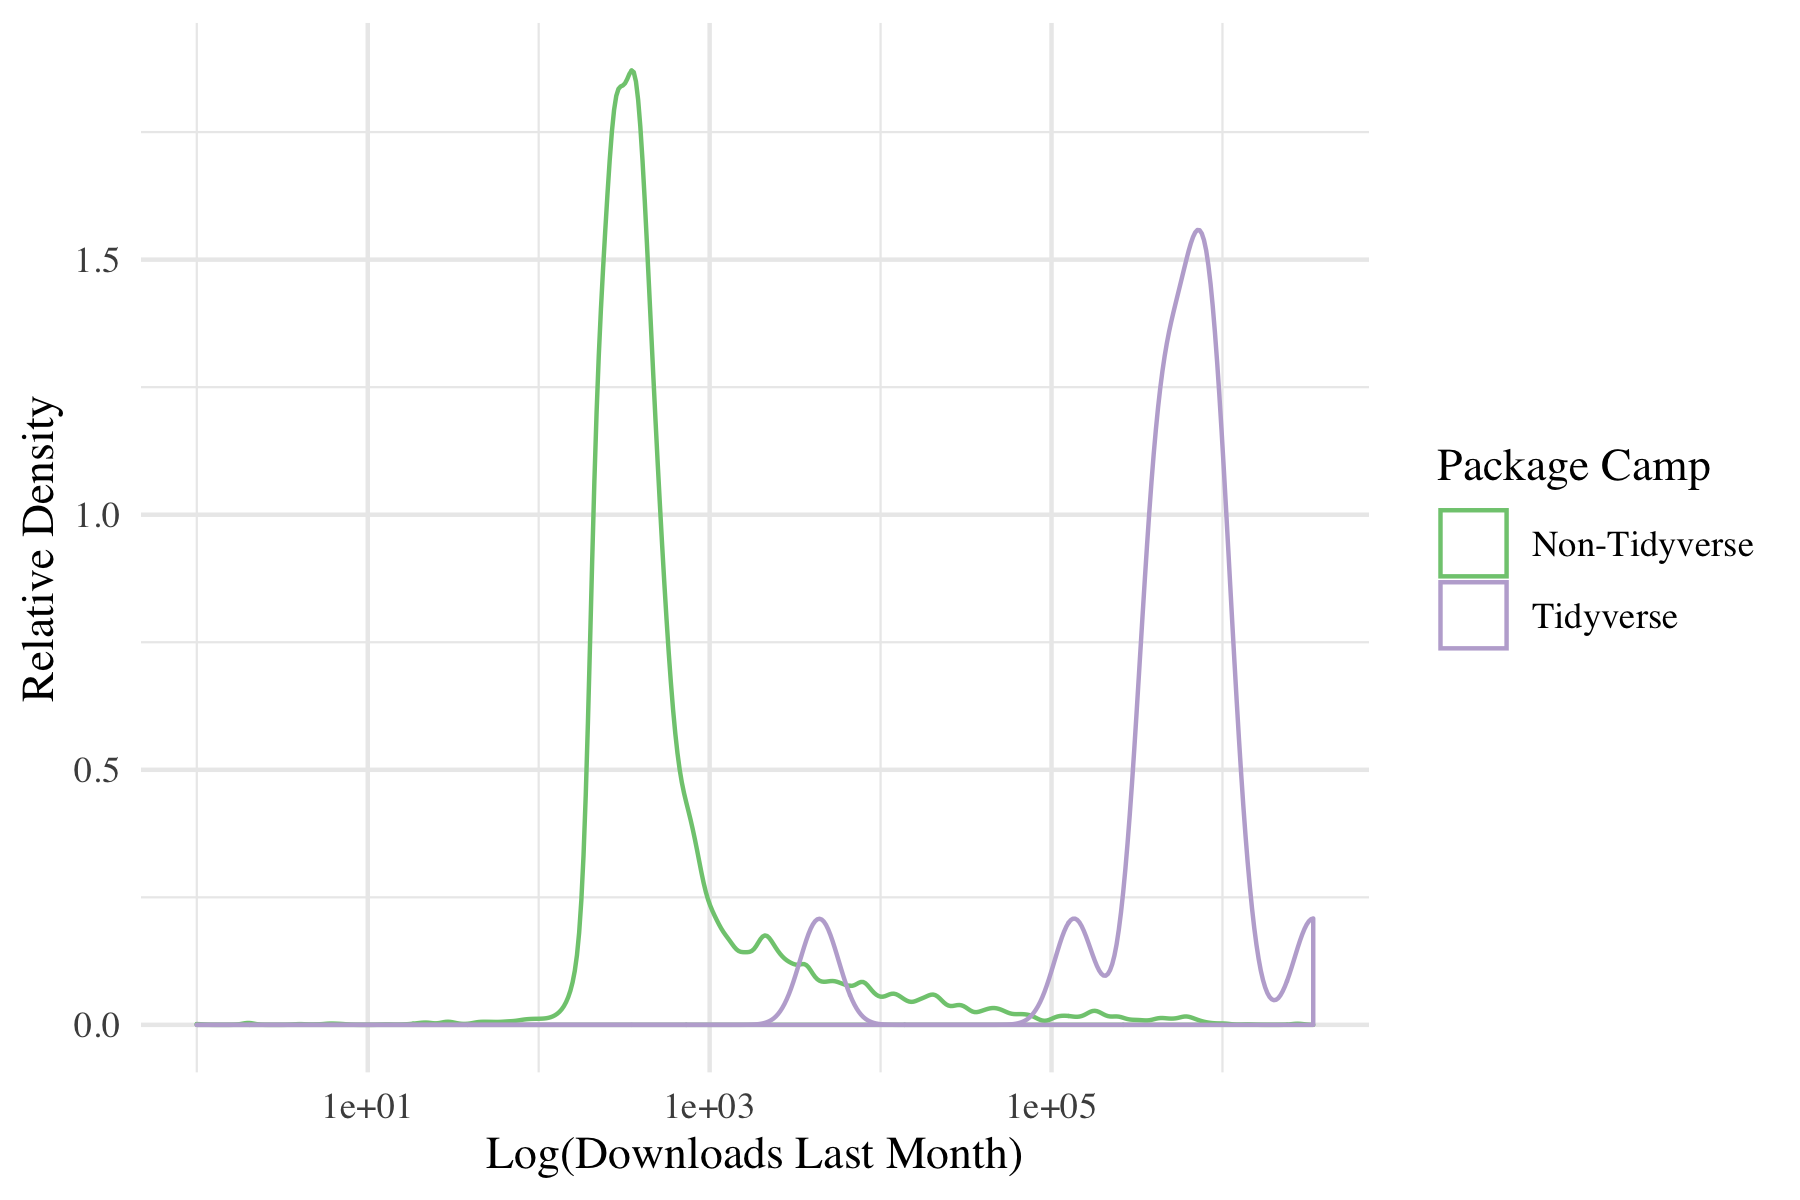
\includegraphics[width=.7\linewidth]{figures/downloads_by_camp.png}
    \captionsetup{width=0.8\textwidth}
    \caption*{Relative density of log (base 10) usership of R software packages in the tidyverse (n = 17, $\mu$ = 755,065) and non-tidyverse (n = 15,227, $\mu$ = 6868).}
    \label{fig:users}
\end{figure}

With this sample of 17 packages from each development community, I then take a census of all exported functions (i.e. those that are available to users) in the packages. In total, this sample includes over 2,200 functions, with 1,500 exported from one of the 17 tidy packages. I then pass each of these functions through an algorithm that extracts variables of interest, described in the next subsection, from the relevant help-files.

\subsubsection{Analysis} \label{sec:met-analyze} \hspace{10pt} The data is collected at the package-level and function-level. My choices of measures to extract from this documentation are a result of my interviews---I've summarized the justification for each of these choices below, alongside discussion from my interviewees.

For package-level documentation, I collect data on two outcomes of interest: whether the package has a \textit{master help-file} accessible by the same help syntax used to seek resources about functions and the \textit{number of vignettes} that the package provides. Accessible master help-files provide a brief introduction into the motivations for using a package, the language and common principles utilized throughout, and directions to find more information on its usage and authorship. Interviewee $A$ started off her answer, when asked about practices for effective documentation, by saying ``one of my pet peeves is packages that don’t have overall documentation.'' Supporting the utilization of my first measure, this interviewee emphasizes the importance of ``providing a general roadmap of what the package is for.'' In regard to my second measure, vignettes are ``a long-form guide to [a] package... [that] can describe the problem that [a] package is designed to solve, and then show the reader how to solve it'' \cite{wickham2015r}. Interviewee $A$ argued that ``multiple types of documentation are very helpful,'' in that the format that works for one learner may be different for another. While this interviewee argued that ``in this day and age, when people want to figure out how to do something, I think they’re a bit more used to clicking around a website'' than reading through plain-text help-files, interviewee $B$ similarly noted that ``the concept of the vignette was really important for making packages more accessible.'' Both of these resources provide a higher-level and more accessible introduction to a package, and the availability of these resources is highly consequential for user understanding.

An arguably greater share of user interaction with documentation happens at the function level. By executing \texttt{?function-name} in the console, users can interact with a relatively standardized, function-specific document (a \textit{help-file}) that describes the purpose of the function, format of user inputs, related functions, and examples. These documents are minimally formatted, containing largely plain text, aside from bolded section headings and links to related help-files. An example help-file is shown in Appendix \ref{fig:ex-help}. While the structure of these help-files is relatively consistent across packages, the amount of content included in these sections, as well as the relative proportion of content devoted to each subsection, varies greatly. Specifically, in my analysis, I focus on the \textit{total character count}, \textit{number of examples}, \textit{number of comments explaining examples}, and \textit{number of functions per help-file}. Interviewee $B$ argued that ``it's really important that you include enough text to actually explain what the function is for and how it's used.'' While basic syntax makes up some portion of the total character count in a help-file, the presence of exposition drastically inflates this number. In general, then, I assert that a greater character count implies a more substantial explanation of functionality and usage and is one useful measure of documentation completeness. While the structure of these help-files is largely standardized, there is significant variation in the number of examples. Examples offer concrete demonstrations of function usage, and are an important element developing a more complete understanding of a function's usage. Interviewee $A$ stated that ``good examples that don’t require domain knowledge or familiarity with a specific dataset'' are an important element of function-level documentation. Further, these examples allow for comments intended to explain the reasoning and intuition behind decisions made within the examples. Interviewee $B$ argued that comments explaining examples are necessary in order to ``make writing any examples worth [the developers'] time." I thus posit that these comments are another important indicator for accessibility and effectiveness of help-files. Finally, while help-files are function-specific in the sense that they can only be evoked using specific functions, several closely-related functions can share one help-file. Interviewee B argued that ``linking between functions [within documentation] is another way'' to make code libraries more accessible. I thus assert that effective documentation elicits the interconnections between functions, and thus that related functions ought to be embedded within the same help-file when applicable.

Based on the differences in representation of gender minorities within the tidyverse and non-tidy development communities and the supply-side mechanisms of gendered occupational segregation described in Section \ref{sec:scholarly}, I present the following hypotheses. Initially, as for package level documentation,

\begin{itemize}
	\item \textit{Hypothesis 1(a):} A larger proportion of packages will provide master help-file in tidy packages than in non-tidy packages.
	\item \textit{Hypothesis 1(b):} Tidy packages will provide a greater mean number of vignettes than non-tidy packages.\footnote{It is important to note here that vignettes were developed as part of the tidyverse ecosystem. An additional mechanism alternative to gender (or gender-conscious) representation within the development community might be that tidy packages are more likely to incorporate this form of documentation due to institutional affiliation.}
\end{itemize}

As for function-level documentation,

\begin{itemize}
	\item \textit{Hypothesis 2(a):} The mean character count of function help-files from tidy packages will be greater than that from non-tidy packages.
	\item \textit{Hypothesis 2(b):} The mean number of examples in function help-files from tidy packages will be greater than that from non-tidy packages.
	\item \textit{Hypothesis 2(c):} The mean number of comments explaining examples in function help-files from tidy packages will be greater than that from non-tidy packages.
	\item \textit{Hypothesis 2(d):} The mean number of functions per help-file will be greater for documentation from tidy packages than that from non-tidy packages.
\end{itemize}

In carrying out significance tests, I use a two-sided significance level $\alpha = .05$.

These hypotheses do not necessarily assert causality related to gender representation. Instead, I intend to argue that documentation practices and gender representation are in constant dialogue. In one way, effectively (and by extension, inclusively) written documentation contributes to an alleviation of the supply side mechanisms discouraging gender minorities' ``self-selection'' away from statistical computing in the tidyverse. Conversely, the greater representation of gender minorities in the tidyverse development community, who are more likely to have encountered documentation written with inclusivity in mind, normalizes and solidifies the expectation of effective and inclusive documentation practices. While the class of object analysis serves only to establish these correlations quantitatively, I explore the arguments for the mechanisms driving them more thoroughly in Section \ref{sec:qual} and \ref{sec:disc}.


\section{Results}\label{sec:results}

\subsection{Qualitative Interviews}\label{sec:results-qual}

\subsubsection{Confounding Factors} \hspace{10pt} Throughout the course of interviewing, these developers mention several other mechanisms that might lead to differences in the appearance of documentation between tidyverse packages and other packages. I begin by noting each of these proposed mechanisms, regardless of the frequency with which they came up, in order to most generously acknowledge the role that other factors, some of which have been previously discussed, might play in driving this association between gender representation and documentation practices.

A principal mechanism that the interviewees suggest might be driving these differences in documentation practices between development communities are the increased resources available to the core developers of the tidyverse team, as compared to other open-source developers. Interviewee $A$ noted that ``100\% of their day, 100\% of their work is package development, so they spend a lot more time and a lot more energy than people who develop packages, but that’s not their only job.'' Given that the tidyverse team's principal work is open-source package development, they can devote more time and energy to the overall process than many others who write open-source software, say, after working some other (paid) development job. When this additional time is available, this interviewee suggests, it is more likely to be spent on documentation than building out code functionality. 

Both interviewees also pointed out that the tidyverse team is in much closer communication with each other than the R development community outside of the tidyverse. As interviewee $A$ noted, ``if there’s something that’s working for one package, there tends to be a decision to do the same thing for other packages as well.'' This uniformity in documentation structure and appearance within the tidyverse, then, could be a result of the close connections between developers in the tidyverse team, ``who are all working under the same roof,'' resulting in quicker dissemination of practices within the community than outside of it. Interviewee $B$ shared this sentiment, noting that, within the tidyverse team, ``there’s a strong culture of information sharing of good development practices.'' These structural influences, then, allow documentation within the tidyverse to share a common structure and quality.

At the same time, though, both interviewees also note that many developers outside of the tidyverse community make use of the many packages developed by the tidyverse team. In addition to writing tools for R users, the tidyverse team has developed many popular tools for R package developers, including the \textit{pkgdown}, \textit{usethis}, \textit{roxygen2}, and \textit{devtools} packages, each of which automates or simplifies development and documentation workflows. As interviewee $A$ noted, ``when a decision is made about ‘this is a good idea,’ that gets implemented in either \textit{pkgdown} or a package like \textit{usethis}... then it becomes a lot easier for others to adopt the same practices.'' In this way, documentation from developers outside of the tidyverse team comes to look more similar to documentation written by the tidyverse team. Similarly, as interviewee $B$ noted, ``What has made it easy for other people to adopt these practices [shared by the tidyverse team] is that then they built packages for making it easier'' to write documentation. In this way, the organizational influence on documentation practices is weakened, as developers outside of the core team still have access to the tools that make writing effective documentation easier. Interviewee $A$ also noted that R developers outside of the tidyverse team still ``probably take cues about writing documentation from Hadley’s \textit{R Packages},'' a book written the tidyverse founder Hadley Wickham that has become the gold standard manual for R package development. These cues come both in the form of the general approach and language that is exemplified in \textit{R Packages} as well as the many references to the aforementioned packages developed by the tidyverse team \cite{wickham2015r}.

An additional mechanism by which interviewee $A$ proposed that documentation practices might differ are the actual principles by which many tidyverse packages are written. While I propose that the effect predicted in Hypothesis $2(d)$ is reflective of more effective documentation practices, this interviewee also adds that many packages within the tidyverse contain functions that are more related to each other than functions provided by packages outside of the tidyverse. ``There probably are more linked functions within the tidyverse than in some other packages... tidyverse packages, from a design perspective, are designed in a way that'' the value of the package functionality lies more in the connections between functions than in other R packages. A forthcoming publication by the tidyverse team states that ``carefully designing functions so that the inputs and outputs align'' and ``identifying the atoms of a problem and the ways in which [their solutions] might be composed to solve bigger problems'' are underlying principles of the design philosophy of the tidyverse \cite{wickham2020tidyverse}. In this way, the greater interconnections between functions evoked in documentation within the tidyverse could be due to the design principles underlying the code itself.

\subsubsection{Supply-Side Mechanisms} \hspace{10pt} In addition to the alternative mechanisms for the association between gender representation and documentation practices (via the tidyverse) mentioned above, though, the interviewees elaborated on the differential effect of poorly written documentation for gender minorities, and the arguments for a relationship beyond correlation between representation of gender minorities in development communities and the quality of documentation resulting from those communities.

Both of these interviewees use the language of a ``user base'' when describing the implications for poorly written documentation. Their arguments presuppose a pipeline model, where gender minorities (and minorities in other identities) are better represented in a pool of potential developers, and ``gradually drop out'' as these learners move farther along in their educational and career paths. As interviewee $A$ said, ``I do believe that writing better documentation is helpful for capturing a greater percentage of your user base, which inevitably, hopefully, will mean you’re also capturing the people who are most likely to fall through the cracks at the first step.'' Interviewee $B$ conceptualized this process of leakage in a similar way: ``writing better documentation will inevitably increase your user base, and it is more likely to then, you know, capture certain subpopulations there too.'' Interviewee $A$ pointed to students' first interactions with R in introductory classes as this pivotal first step: ``If it’s a student [who is interacting with poorly written documentation], they’re not going to enjoy it, and then they’ll remember statistics as something annoying they had to do... You probably lost your customer, if you will.'' This same interviewee argued that these implications of documentation practices for inclusivity move beyond the classroom, saying that if these prospective users ``otherwise wouldn’t see themselves as stereotypical programmers... from a welcoming or inclusive perspective, again, it depends on whether they feel like `is this something I can master?' or not.'' After reflecting on literature in learning theory, she states, ``There has to be a relationship between an accessible nature of your documentation and whether or not someone who lands on your documentation page can think `yeah, this is something I can do.'\thinspace'' If the measures used in this study, then, are appropriate markers of accessibility, the mechanisms for greater representation of gender minorities within tidyverse development communities become clear.


Interviewee $A$ also reflected on how diversity improvement efforts are now structurally embedded in the production of documentation. Starting in early 2019, the tidyverse now hosts a ``tidyverse developer day'' (\textit{tidy-dev day}) at the conclusion of ``rstudio::conf'' and ``useR!'', two prominent R user conferences. With a stated goal to ``nurture regular contributors,'' the event provides a welcoming and inclusive environment for new contributors to the open-source tidyverse codebase, focusing on increasing diversity within the development community. As an advertisement for the first session promised, ``The tidyverse team will be there, so we can help you hit the ground running and/or get over any stumbling blocks that you encounter'' \cite{averick_tidyverse_2018}. This interviewee notes, too, ``When we’re going through and tagging issues as appropriate for tidy-dev day, there are a lot of issues that get tagged for documentation. This event also has a goal of increasing diversity, so in terms of who gets to attend it, there’s a deliberate effort to have a diverse crowd... Many of the issues they work on are documentation-related.'' In this way, representation of work done by contributors with minority identities within the tidyverse codebase becomes uniquely amplified in the production and revision of code documentation.

\subsection{Class of Object Analysis}\label{sec:results-coa}

In general, my analyses support the hypotheses presented in Section \ref{sec:met-analyze}.

As for package-level resources, I initially find that packages in the tidyverse are statistically significantly more likely (52\%) to provide vignettes in their documentation ($p = .005$). Further, packages from the tidyverse were 29\% more likely to provide master help-files than the sampled non-tidy packages, though this difference in proportions is not statistically significant, ($p = .143$). Thus, I find that Hypothesis 1 is generally supported (though only directionally for $1(b)$). 

My findings for function-level resources, in regard to hypotheses $2(a)$, $2(b)$, $2(c)$, and $2(d)$, are similar. On average, function help-files in the tidyverse contain 1468 more characters than those from non-tidy packages ($p < .001$). While the difference is not statistically significant, function help-files from tidy packages have, on average, .12 more examples than those from non-tidy packages ($p = .462$). In regard to comments, though, function help-files from the tidyverse have a statistically significantly greater mean number of comments ($\mu = 4.12$) than those from non-tidy packages ($\hat{\mu} = 1.73$, $p < .001$). Finally, the mean number of functions per help-file in the tidyverse ($\mu = 7.14$) is statistically significantly greater than that in non-tidy packages ($\hat{\mu} = 5.97, ~p < .001$). Thus, altogether, I find that Hypothesis 2 is supported (though only directionally for $2(b)$), and thus that help-files from functions in the tidyverse align with the proposed principles for effective and inclusive documentation more so than those from non-tidy packages.



\section{Discussion}\label{sec:disc}

Future work on this topic can further the arguments made here in several ways. While experimentation evaluating the validity of this argument specifically may not be ethical, future work should strive to more thoroughly and rigorously evaluate code documentation practices as a causal mechanism for greater representation of gender minorities in computing. Namely, the differences in cultural and structural setting between the tidyverse and other R development communities go far beyond code documentation practices---demonstrating this same effect in a variety of computing contexts in which these same cultural and structural factors are reversed or not at play could strengthen the argument for this causal mechanism. Further, the line between tidyverse and non-tidyverse development is not an obvious one. I've referred to tidyverse packages as those included in the core tidyverse, as well as those refereed to on tidyverse publications as closely adjacent to the tidyverse. As the interviewees discussed, though, the tidyverse (as a toolkit) has a significant impact on the way that package development, and especially the writing of documentation, is carried out in other R development communities. Beyond those that just make use of tidyverse tools to write documentation, many package developers explicitly align with tidyverse principles in their development practices. In this way, alignment in development practices with the tidyverse exists on spectra far beyond a binary. Lastly, I note that the use of the term ``community'' in this paper is coarse, and may elicit the sense that these two development groups are similarly interconnected. In reality, the group developing the tidyverse is more often referred to as a ``team'' than a ``community'' by my interviewers, due to many of the group members' common professional affiliation with RStudio. On the other hand, those developing outside of the tidyverse framework make up a heterogeneous and decentralized group. Between these two groups, then, we see very different mediums for communication---while the tidyverse team is largely in frequent, direct communication, the primary mechanism for norm-setting of documentation practices outside of the tidyverse, if not making use of resources developed by the tidyverse, is likely mimicry of others' documentation.

Throughout this paper, I have argued that code documentation in the tidyverse is written more effectively and inclusively than other R code documentation, and that this is meaningful for understanding gender representation in the user community. Initially, I traced the literature articulating supply-side mechanisms for occupational segregation, showing that the work of gender minorities in STEM is subjected to greater scrutiny than their cisgender men counterparts. Further, too, gender minorities in these fields are more likely to incorporate this negative feedback, as well as their awareness of masculine elements of their physical surroundings, into their self-perceptions of their competence and identity alignment with the stereotypical worker. Collectively, these mechanisms coalesce into a system of exclusion discouraging gender minorities from pursuing careers in some STEM fields. I argued that these mechanisms are at play in the context of statistical computing, which incorporates methodological and cultural elements from many STEM fields and, further, that code documentation in statistical computing settings is capable of both delivering feedback about competence and transmitting norms about the stereotypical worker. Next, through interviews with women in these fields, I developed a set of measures to quantify the effectiveness and inclusiveness of code documentation, and analytically showed that code documentation from the tidyverse is more effectively and inclusively written than code outside of the tidyverse. These interviews also allowed me to more thoroughly scrutinize this association between gender minority representation in the tidyverse and the increased quality of documentation arising from the community. The interviewees articulated several confounding factors, as well as supply-side mechanisms, relating these two phenomena---namely, I argue that increased documentation effectiveness and inclusivity are a likely mechanism for the greater representation of gender minorities in tidyverse development communities, and also that, in turn, this greater representation contributes to more effectively and inclusively written documentation. That said, the confounding factors highlighted by the interviews are also plausible mechanisms driving this association, and the evidence provided is not sufficient to fully articulate a causal mechanism in either direction. 


\subsection*{Acknowledgements}

Many thanks to my two interviewees, whom graciously offered their time and perspective. Thank you to Dr. Kjersten Whittingon for her mentorship, advocacy, and valuable thoughts throughout the writing process. Lastly, many thanks to Dr. Kelly McConville and Dr. Andrew Bray for their insights on sampling strategies and inference. 

% add the bibliography
\clearpage
\bibliographystyle{plain}
\bibliography{sources.bib}

% and then the appendix!
\clearpage
\appendix
\section{Appendix}\label{sec:appendix}

\subsection{Example Function Help-file}\label{fig:ex-help}

\begin{figure} [!htb]
    \centering
    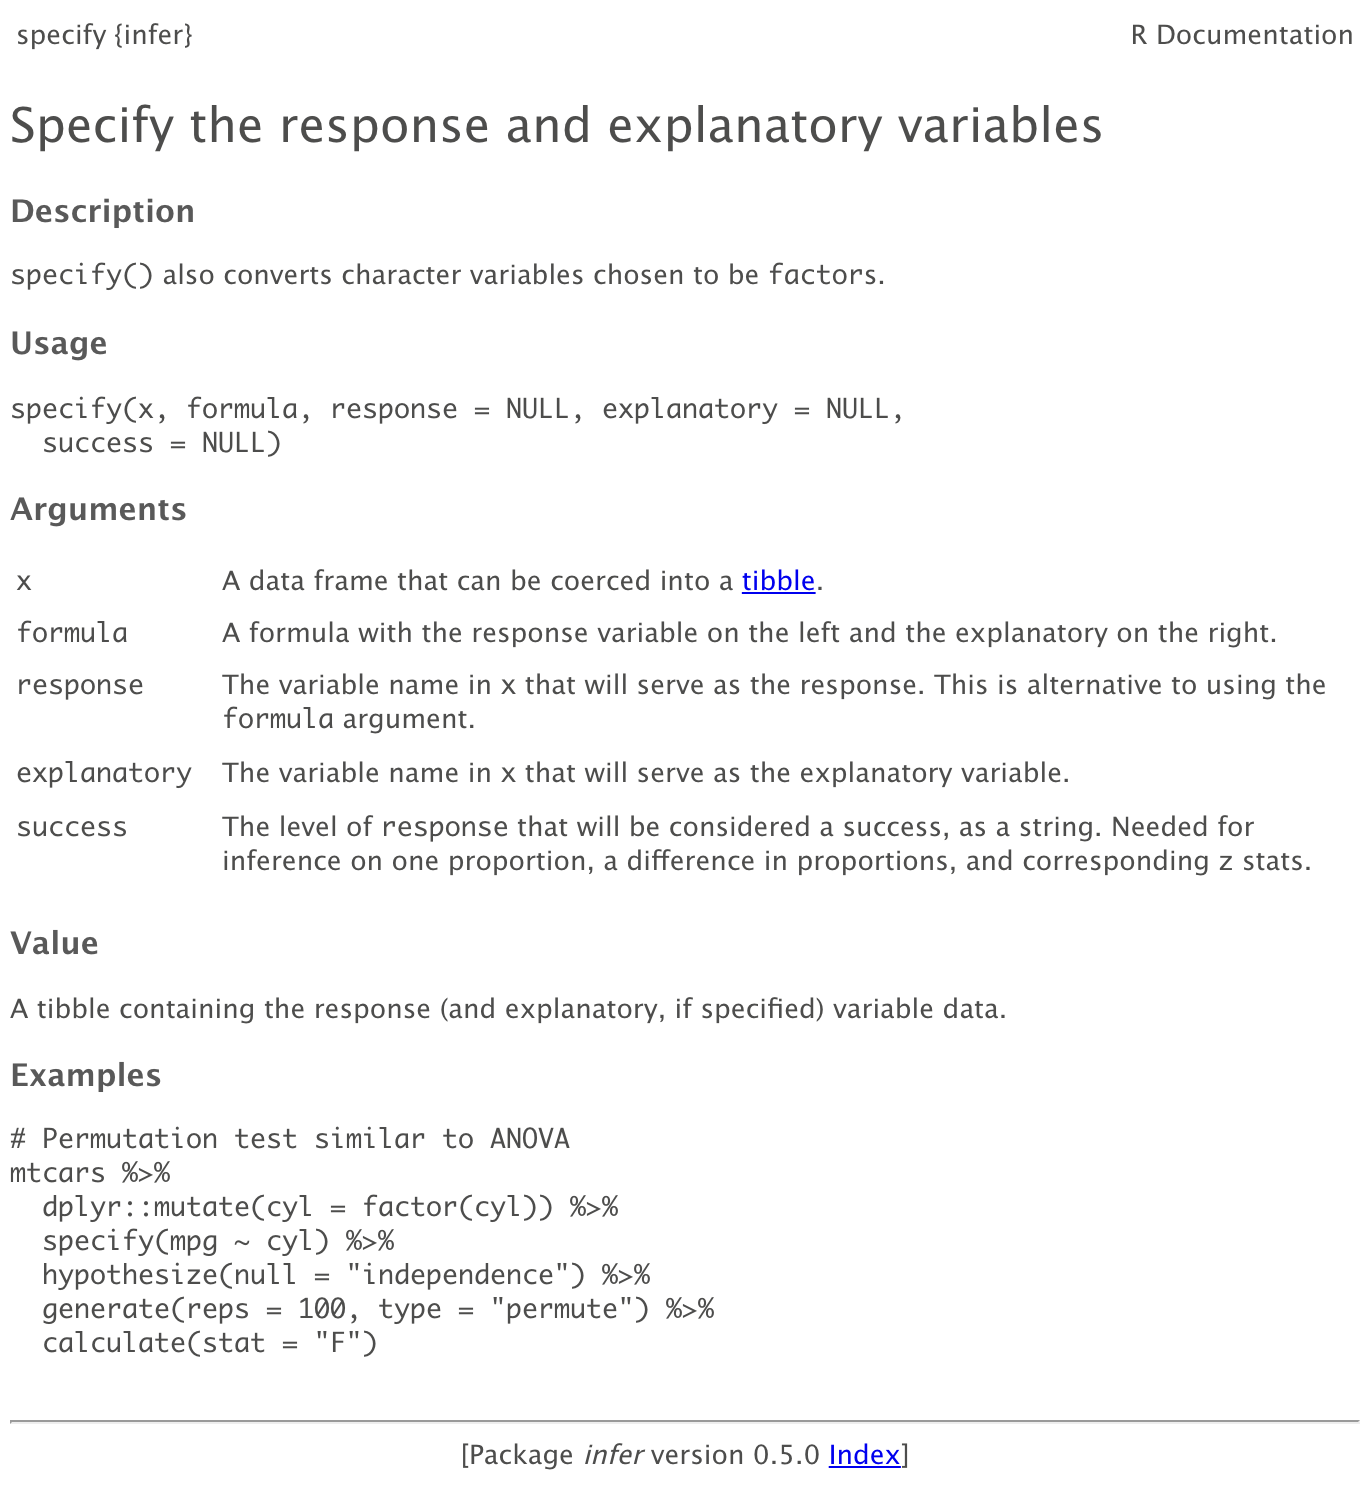
\includegraphics[width=.9\linewidth]{figures/ex_help.png}
    \caption*{A typical example function help-file, describing the \textit{specify} function from version 0.5.0 of the \textit{infer} R package. Function help-files often contain a basic description of the function, the syntax for executing the function, the format of user inputs and outputs, and, often, a practical example demonstrating usage.}
\end{figure}

\clearpage

\subsection{Semi-Structured Interview Protocol}\label{sec:interview}

\begin{itemize}
    \item What makes documentation effective?
    \item What have conversations with (other) tidyverse developers about documentation practices looked like? 
    \item Were there disagreements about any practices?
    \item Is documentation written differently within the tidyverse versus outside of it? (How so? Why might that be?)
    \item What are the consequences of ineffective documentation?
    \item Do gender minorities interact with documentation differently? How so?
    \item How do the demographics of the tidyverse community compare to those in the greater R community?
    \item How do the demographics of the tidyverse community differ from those in other user communities you've been a part of?
    \item I’ve found so far that tidyverse packages are more likely to have package-level help-files, and that function-level help-files from the tidyverse have a greater character count, more examples, more comments per example, and more references to related functions than help-files from non-Tidy libraries. Is this surprising? (What mechanisms might be driving these differences?)
\end{itemize}


\end{document}
